%%%%%%%%%%%%%%%%%%%%%%%%%%%%%%%%%%%%%%%%%%%%%%%%%%%%%%%%%%%%%%%%%%%%%%%%%%%%%%%%%%
\begin{frame}[fragile]\frametitle{}
\begin{center}
{\Large Open AI Gym}
\end{center}
\end{frame}

%%%%%%%%%%%%%%%%%%%%%%%%%%%%%%%%%%%%%%%%%%%%%%%%%%%%%%%%%%%%%%%%%%%%%%%%%%%%%%%%%%
\begin{frame}[fragile]\frametitle{Open AI Gym}

\begin{center}

\includegraphics[width=0.4\linewidth,keepaspectratio]{rl59}
\end{center}

\begin{itemize}
\item Most standard and popular RL task simulation package
\item Has popular Environments which many RL Algorithms libraries support/import
\item gym API are adopted by even rival simulation packages
\end{itemize}

\end{frame}

%%%%%%%%%%%%%%%%%%%%%%%%%%%%%%%%%%%%%%%%%%%%%%%%%%%%%%%%%%%%%%%%%%%%%%%%%%%%%%%%%%
\begin{frame}[fragile]\frametitle{Setup}

\begin{itemize}
\item Not officially supported on Windows, but ok on Linux and Mac
\item Need Visual C++ build tools (Windows) and conda (py 3.9)
\item Create conda virtual env, activate it
\item \lstinline|conda install -c conda-forge gym-all|
\item Start using by \lstinline|import gym|
\end{itemize}

\end{frame}

%%%%%%%%%%%%%%%%%%%%%%%%%%%%%%%%%%%%%%%%%%%%%%%%%%%%%%%%%%%%%%%%%%%%%%%%%%%%%%%%%%
\begin{frame}[fragile]\frametitle{CartPole}

\begin{itemize}
\item Learn how to move the cart in the CartPole environment to maximize the duration (max 10s) the pole stays upright
\item Environment: Cart and Pole
\item Action: Move cart
\item Reward: Duration
\end{itemize}

\begin{lstlisting}
import gym
env = gym.make("CartPole-v1")
env.reset() # to initial state, starts simulation
env.render() # shows graphical view, cant close by cross click
env.close() # force close
\end{lstlisting}

\end{frame}

%%%%%%%%%%%%%%%%%%%%%%%%%%%%%%%%%%%%%%%%%%%%%%%%%%%%%%%%%%%%%%%%%%%%%%%%%%%%%%%%%%
\begin{frame}[fragile]\frametitle{Exercise}


\begin{lstlisting}
# Import gym in this cell

# Create the BipedalWalker-v3 environment and store it in a variable called env

# Reset the simulation to its initial state (this will start the simulation)

# Visualize the initial state
\end{lstlisting}

\end{frame}

%%%%%%%%%%%%%%%%%%%%%%%%%%%%%%%%%%%%%%%%%%%%%%%%%%%%%%%%%%%%%%%%%%%%%%%%%%%%%%%%%%
\begin{frame}[fragile]\frametitle{CartPole}

\begin{itemize}
\item Reset returns initial state, called Observations, 4 elements

\begin{center}
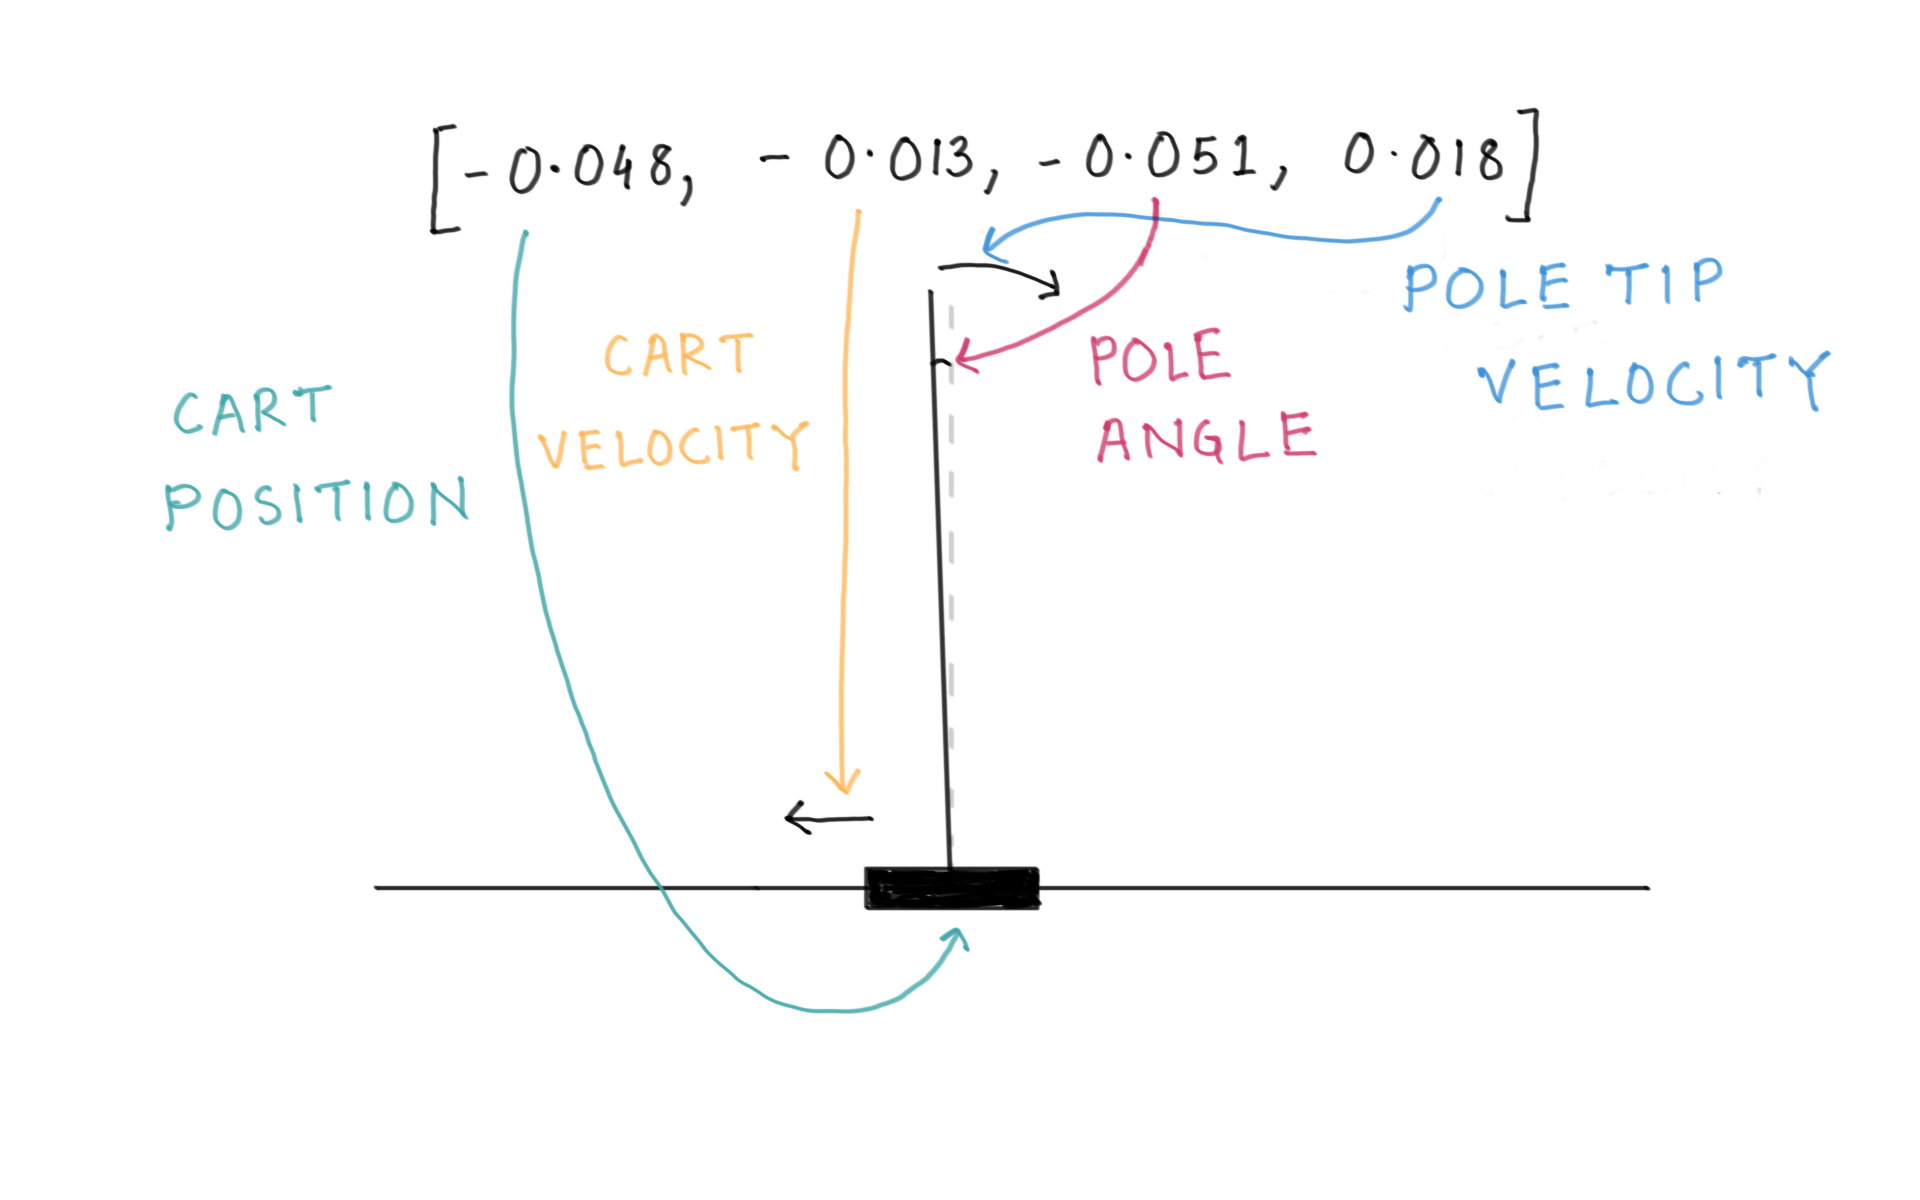
\includegraphics[width=0.5\linewidth,keepaspectratio]{rl60}
{\tiny (Ref: Fast RL course - Dibya Chakraborty)}
\end{center}

\item Are Observations continuous or discrete, scalar/vector/tensor, data-type?
\item `Box` for continuous, `(4,)` for 4 dimensional vector, lower range is first element in array, higher is the 2nd element. Data type is np.float32
\end{itemize}

\begin{lstlisting}
obs = env.reset() 
print(env.observation_space)

Box([-4.8000002e+00 -3.4028235e+38 -4.1887903e-01 -3.4028235e+38], [4.8000002e+00 3.4028235e+38 4.1887903e-01 3.4028235e+38], (4,), float32)
\end{lstlisting}


\end{frame}

%%%%%%%%%%%%%%%%%%%%%%%%%%%%%%%%%%%%%%%%%%%%%%%%%%%%%%%%%%%%%%%%%%%%%%%%%%%%%%%%%%
\begin{frame}[fragile]\frametitle{CartPole}

\begin{itemize}
\item Action is taken every 0.025 sec, to move right or left.
\item After reset, Env waits to receive action from Agent.
\item Here, actions are Discrete(2): 0,1, they are left and right.
\item Sending action is done by `step` with action in it.
\item Env will then simulate the change, and return the next observation.
\end{itemize}

\begin{center}
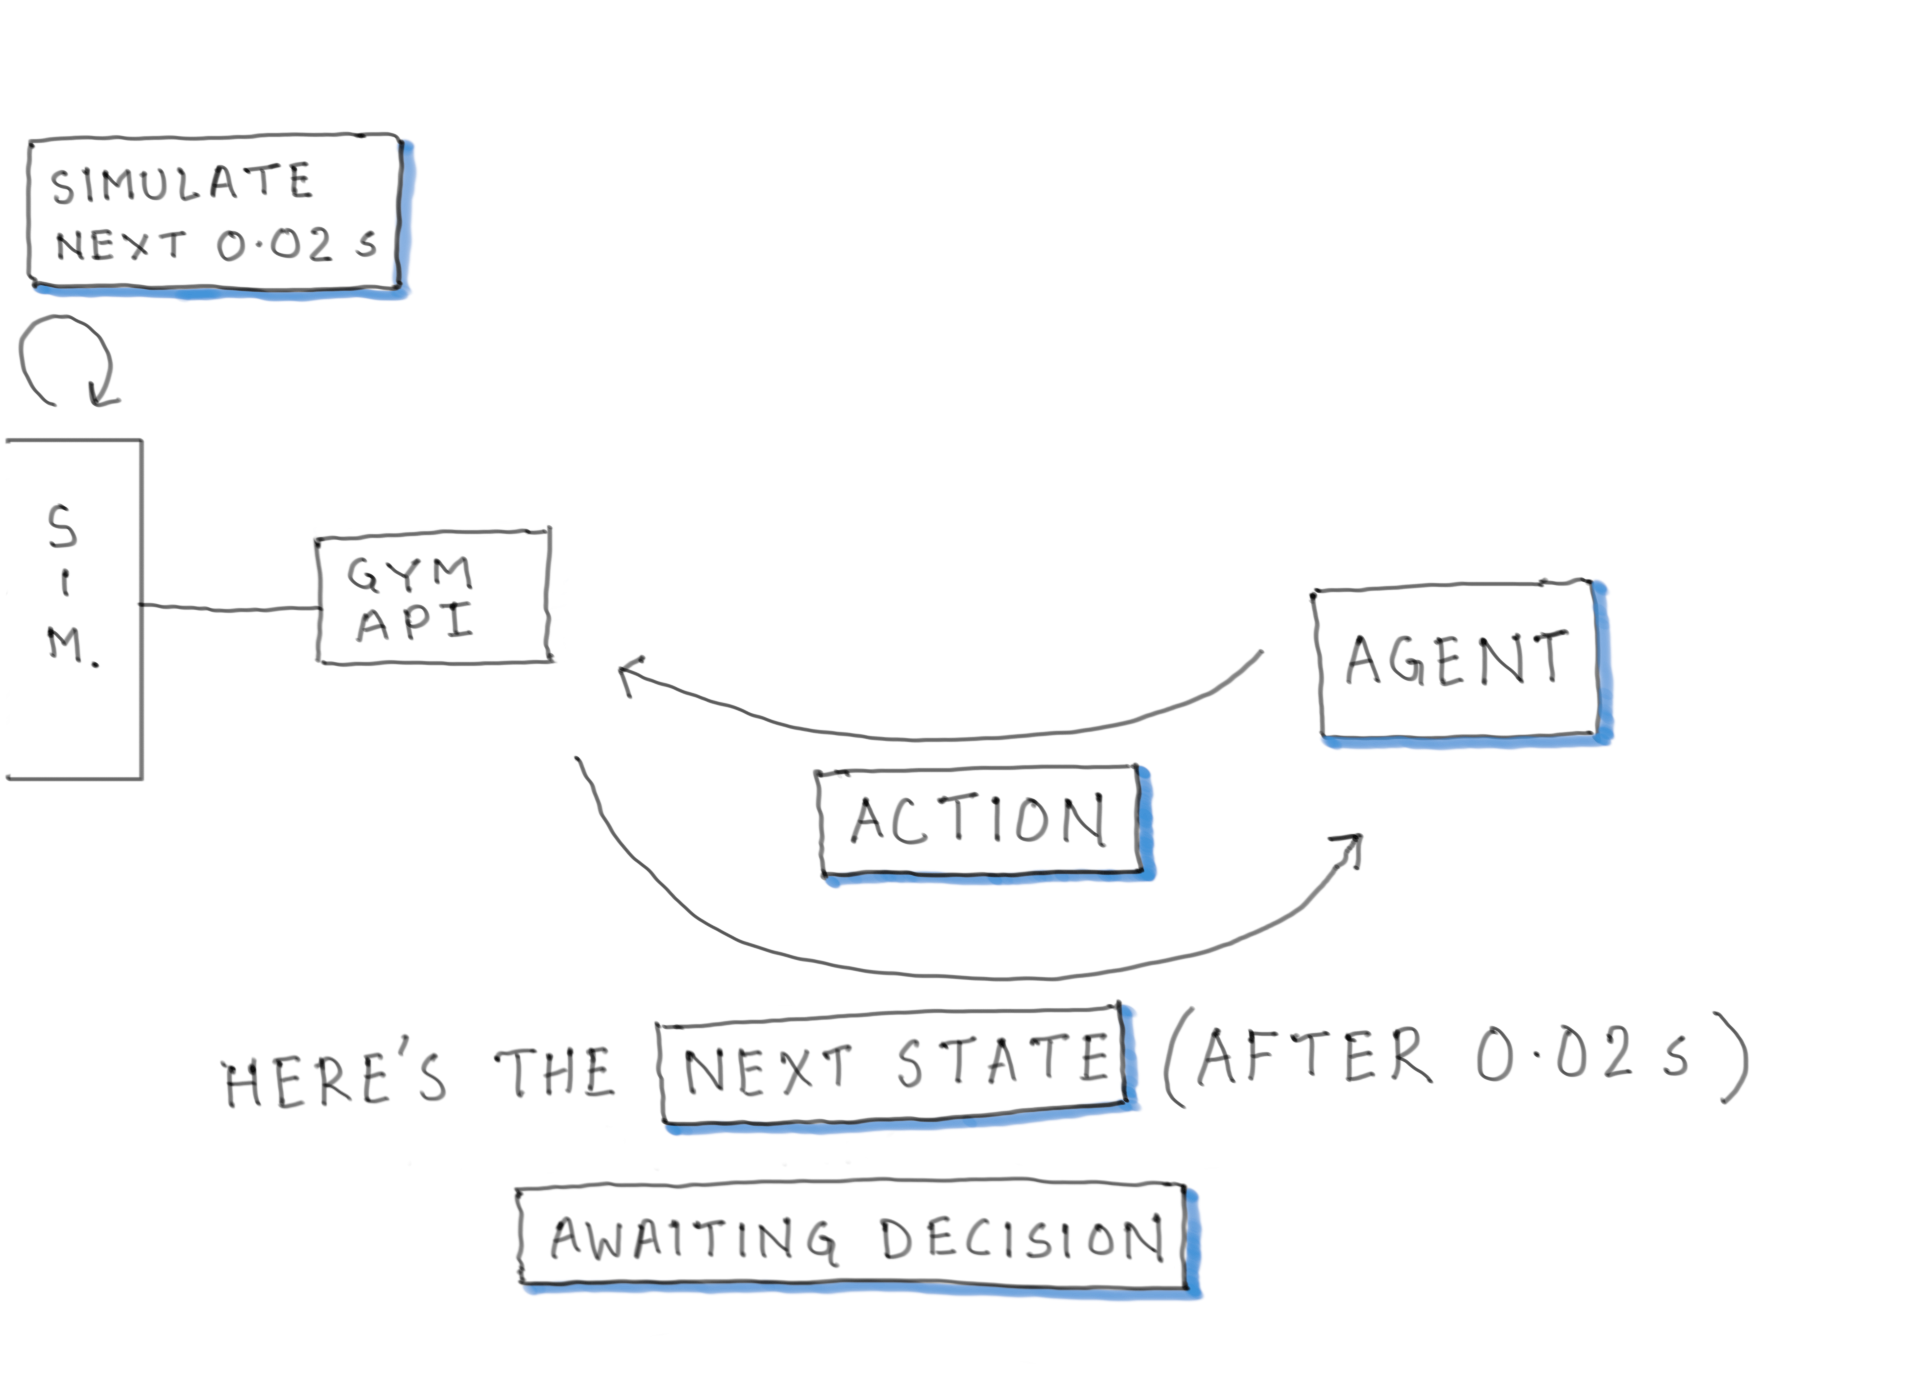
\includegraphics[width=0.3\linewidth,keepaspectratio]{rl61}
{\tiny (Ref: Fast RL course - Dibya Chakraborty)}
\end{center}

\begin{lstlisting}
new_obs, _, _, _ = env.step(0) # left
[ 0.03689718 -0.15012246  0.00797674  0.31285113]
new_obs, _, _, _ =  env.step(1) # right
[-0.02508183, -0.22606609,  0.0646681 ,  0.3370987 ]
\end{lstlisting}


\end{frame}

%%%%%%%%%%%%%%%%%%%%%%%%%%%%%%%%%%%%%%%%%%%%%%%%%%%%%%%%%%%%%%%%%%%%%%%%%%%%%%%%%%
\begin{frame}[fragile]\frametitle{CartPole}

Taking many actions in a loop

\begin{itemize}
\item reset() the env
\item take action 0 in a loop (push cart to the left)
\item call render() after every step
\item render shows that the cart is moved to left
\end{itemize}

\begin{lstlisting}
obs = env.reset()
for _ in range(30):
    print(obs)
    obs, _, _, _ = env.step(0)
    env.render()
\end{lstlisting}


\end{frame}

%%%%%%%%%%%%%%%%%%%%%%%%%%%%%%%%%%%%%%%%%%%%%%%%%%%%%%%%%%%%%%%%%%%%%%%%%%%%%%%%%%
\begin{frame}[fragile]\frametitle{CartPole}

Gym has a Reward function for CartPole
\begin{itemize}
\item If the pole is within +-12 degrees from vertical, reward is +1, else 0
\item Pole must  stay between environment bounds +- 2.4
\item Maximizing the cumulative reward is equivalent to maximizing the number of steps the pole stays upright.
\item $duration=0.02s \times num steps$
\item Maximizing the cumulative reward is equivalent to maximizing the duration the pole stays upright.
\end{itemize}

\begin{lstlisting}
obs = env.reset()
for _ in range(30):
    print(f"Pole angle at step start: {np.degrees(obs[2])}", end=" ")
    obs, reward, _, _  = env.step(0)
    print(f"Reward in this step: {reward}")
Pole angle at step start: -1.9815118943994086 Reward in this step: 1.0
Pole angle at step start: -1.9753829089133865 Reward in this step: 1.0
:		
\end{lstlisting}


\end{frame}

%%%%%%%%%%%%%%%%%%%%%%%%%%%%%%%%%%%%%%%%%%%%%%%%%%%%%%%%%%%%%%%%%%%%%%%%%%%%%%%%%%
\begin{frame}[fragile]\frametitle{CartPole}

\begin{itemize}
\item Episodes decide till what duration the rewards need to be accumulated.
\item In games, the episodes end at Win/Loss/Terminal states.
\item The third element of the return value of env.step(action) indicates if we have reached a terminal state
\item In Cartpole, there is no reward 0, but thats the Terminal state (pole down, boundary touch). Pole is upright and 500 steps are reached, then we win.
\end{itemize}

\begin{lstlisting}
obs = env.reset()
for _ in range(30):
    print(f"Pole angle at step start: {np.degrees(obs[2])}", end=" ")
    obs, reward, done, _  = env.step(0)
    print(f"Pole angle at step end: {np.degrees(obs[2])}", end=" ")
    print(f"Reward in step: {reward}, done: {done}")
		
Pole angle at step start: 2.5225715240513926 Pole angle at step end: 2.5628541577896797 Reward in step: 1.0, done: False
Pole angle at step start: 2.5628541577896797 Pole angle at step end: 2.9540647813957777 Reward in step: 1.0, done: False
Pole angle at step start: 2.9540647813957777 Pole angle at step end: 3.6964366026209015 Reward in step: 1.0, done: False
:		
\end{lstlisting}


\end{frame}

%%%%%%%%%%%%%%%%%%%%%%%%%%%%%%%%%%%%%%%%%%%%%%%%%%%%%%%%%%%%%%%%%%%%%%%%%%%%%%%%%%
\begin{frame}[fragile]\frametitle{CartPole}

Doing multiple episodes
\begin{itemize}
\item Once done is True, we should not take any more actions
\item To collect, call env.reset() if you want to restart the simulation
\end{itemize}

\begin{lstlisting}
for ep in range(5):
    print(f"Episode number is {ep+1}")
    obs = env.reset()
    while True:
        print(f"Pole angle at step start: {np.degrees(obs[2])}", end=" ")
        obs, reward, done, _  = env.step(0)
        print(f"Pole angle at step end: {np.degrees(obs[2])}", end=" ")
        print(f"Reward in step: {reward}, done: {done}")
        if done:
            break
						
Episode number is 1
Pole angle at step start: 1.1183983506183337 Pole angle at step end: 1.1099812877349993 Reward in step: 1.0, done: False
:
Episode number is 2
Pole angle at step start: 0.515380400430025 Pole angle at step end: 0.5154796938477244 Reward in step: 1.0, done: False
:
\end{lstlisting}

\end{frame}